%\documentclass[11pt]{book}
%
%\setlength{\parindent}{0pt}
%\setlength{\parskip}{8pt}
%
%\usepackage{amsmath}
%\usepackage{amssymb}
%\usepackage{hyperref}
%\usepackage{cleveref}
%
%\renewcommand*{\thefootnote}{\fnsymbol{footnote}}
%
%\setcounter{chapter}{3}
%
%\begin{document}
%
%\section*{A Levelized Comparison of \\ Pulsed and Steady-State Tokamaks}
%
%\let\cleardoublepage\relax \tableofcontents \newpage

\chapter{Presenting the Code Results}

\section{Validating Code with other Models}

\newpage 

\subsection{Comparing with the PSFC Arc Reactor}

\begin{figure*}[h!]
    \centering
    \hfill 
    \begin{subfigure}[t]{0.45\textwidth}
        \centering
    \begin{adjustbox}{width=\textwidth}
      \Large
      \input{images/comparisons/arc_B_0_vs_R_0}
    \end{adjustbox}
        \caption{$R_0$ vs $B_0$}
    \end{subfigure}
    \hfill
    \begin{subfigure}[t]{0.45\textwidth}
        \centering
    \begin{adjustbox}{width=\textwidth}
      \Large
      \input{images/comparisons/arc_T_bar_vs_I_P}
    \end{adjustbox}
        \caption{$I_P$ vs $\overline T$}
    \end{subfigure}
    \hfill \hfill ~\\ ~\\ ~\\
    \caption{Arc Model Comparison} ~\\
\end{figure*}

\begin{table}[h!]
\centering  
\caption{Arc Variables}
\hfill
\begin{subtable}[t]{0.4\textwidth}
\centering  
\caption{Input Variables} ~\\
\begin{tabular}{ c|c } 

Input            & Value           \\
\hline
$H$              & 1.8             \\
$Q$              & 13.6            \\
$N_{G}$          & 0.67            \\
$\epsilon$       & 0.3333          \\
$\kappa_{95}$    & 1.84            \\
$\delta_{95}$    & 0.333           \\
$\nu_{n}$        & 0.385           \\
$\nu_{T}$        & 0.929           \\
$l_{i}$          & 0.67            \\
$A$              & 2.5             \\
$Z_{eff}$        & 1.2             \\
$f_{D}$          & 0.9             \\
$\tau_{FT}$      & 1.6e9           \\
$B_{CS}$         & 12.77           \\

\end{tabular}
\end{subtable}
\hfill
\begin{subtable}[t]{0.5\textwidth}
\centering  
\caption{Output Variables} ~\\
\begin{tabular}{ c|c|c } 

Output           & Original         & Fussy.jl        \\
\hline
$R_{0}$          & 3.3              & 3.382           \\
$B_{0}$          & 9.2              & 9.505           \\
$I_{P}$          & 7.8              & 8.766           \\
$\overline n$    & 1.3              & 1.291           \\
$\overline T$    & 14.0             & 16.78           \\
$\beta_{N}$       & 0.0259           & 0.0259          \\
$q_{95}$         & 7.2              & 6.127           \\
$P_{W}$          & 2.5              & 2.215           \\
$f_{BS}$         & 0.63             & 0.5588          \\
$f_{CD}$         & 0.37             & 0.4412          \\
$f_{IN}$         & -              & -             \\
$\volume$         & 141.0            & 157.4           \\
$P_{F}$          & 525.0            & 725.9           \\
$\eta_{CD}$      & 0.321            & 0.3164          \\

\end{tabular}
\end{subtable}
\hfill
\hfill
\end{table}

\newpage

\subsection{Contrasting with the Aries Act Studies}

\newpage 

\subsubsection{Act I -- Advanced Physics and Engineering}

\begin{figure*}[h!]
    \centering
    \hfill 
    \begin{subfigure}[t]{0.45\textwidth}
        \centering
    \begin{adjustbox}{width=\textwidth}
      \Large
      \input{images/comparisons/act_1_B_0_vs_R_0}
    \end{adjustbox}
        \caption{$R_0$ vs $B_0$}
    \end{subfigure}
    \hfill
    \begin{subfigure}[t]{0.45\textwidth}
        \centering
    \begin{adjustbox}{width=\textwidth}
      \Large
      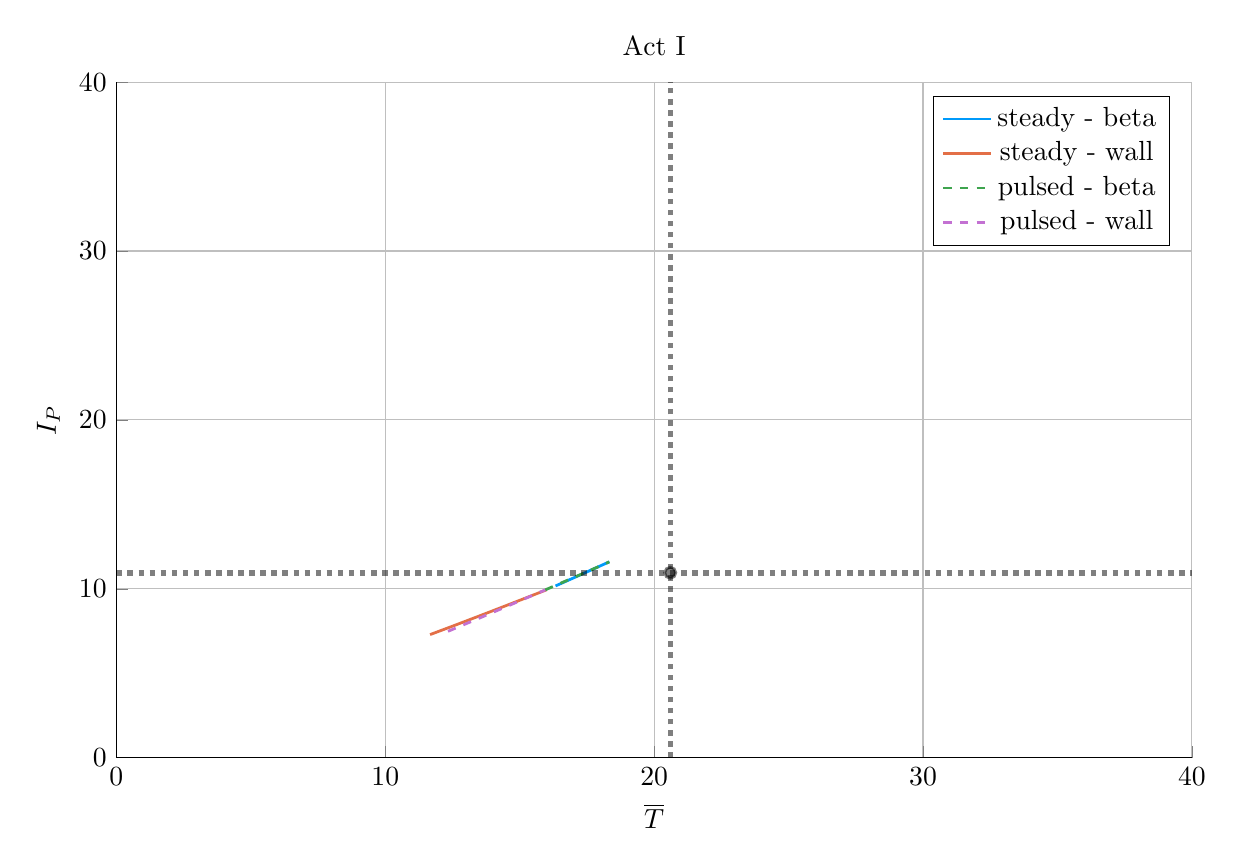
\begin{tikzpicture}[]
\begin{axis}[height = {101.6mm}, ylabel = {$I_P$}, title = {Act I}, xmin = {0.0}, xmax = {40.0}, ymax = {40.0}, xlabel = {$\overline T$}, {unbounded coords=jump, scaled x ticks = false, xticklabel style={rotate = 0}, xmajorgrids = true, xtick = {0.0,10.0,20.0,30.0,40.0}, xticklabels = {0,10,20,30,40}, xtick align = inside, axis lines* = left, scaled y ticks = false, yticklabel style={rotate = 0}, ymajorgrids = true, ytick = {0.0,10.0,20.0,30.0,40.0}, yticklabels = {0,10,20,30,40}, ytick align = inside, axis lines* = left,     xshift = 0.0mm,
    yshift = 0.0mm,
    axis background/.style={fill={rgb,1:red,1.00000000;green,1.00000000;blue,1.00000000}}
}, ymin = {0.0}, width = {152.4mm}]\addplot+ [color = {rgb,1:red,0.00000000;green,0.60560316;blue,0.97868012},
draw opacity=1.0,
line width=1,
solid,mark = none,
mark size = 2.0,
mark options = {
    color = {rgb,1:red,0.00000000;green,0.00000000;blue,0.00000000}, draw opacity = 1.0,
    fill = {rgb,1:red,0.00000000;green,0.60560316;blue,0.97868012}, fill opacity = 1.0,
    line width = 1,
    rotate = 0,
    solid
}]coordinates {
(16.333333333333332, 10.169194435531358)
(16.666666666666668, 10.405057509328124)
(17.0, 10.641905327194731)
(17.333333333333332, 10.87971637136811)
(17.666666666666668, 11.11846917050157)
(18.0, 11.358142407296011)
(18.333333333333332, 11.598714938197329)
};
\addlegendentry{steady - beta}
\addplot+ [color = {rgb,1:red,0.88887350;green,0.43564919;blue,0.27812294},
draw opacity=1.0,
line width=1,
solid,mark = none,
mark size = 2.0,
mark options = {
    color = {rgb,1:red,0.00000000;green,0.00000000;blue,0.00000000}, draw opacity = 1.0,
    fill = {rgb,1:red,0.88887350;green,0.43564919;blue,0.27812294}, fill opacity = 1.0,
    line width = 1,
    rotate = 0,
    solid
}]coordinates {
(11.666666666666666, 7.287903136887)
(12.0, 7.486025430610099)
(12.333333333333334, 7.685696663157812)
(12.666666666666666, 7.886645361110723)
(13.0, 8.08866940687473)
(13.333333333333334, 8.291629426976055)
(13.666666666666666, 8.495414075666067)
(14.0, 8.699964056113311)
(14.333333333333334, 8.905213556979005)
(14.666666666666666, 9.111120468746519)
(15.0, 9.31764336053339)
(15.333333333333334, 9.524758318501357)
(15.666666666666666, 9.732442959434447)
(16.0, 9.940679052729761)
};
\addlegendentry{steady - wall}
\addplot+ [color = {rgb,1:red,0.24222430;green,0.64327509;blue,0.30444865},
draw opacity=1.0,
line width=1,
dashed,mark = none,
mark size = 2.0,
mark options = {
    color = {rgb,1:red,0.00000000;green,0.00000000;blue,0.00000000}, draw opacity = 1.0,
    fill = {rgb,1:red,0.24222430;green,0.64327509;blue,0.30444865}, fill opacity = 1.0,
    line width = 1,
    rotate = 0,
    solid
}]coordinates {
(15.948125117373092, 9.933500150990564)
(15.9481251173731, 9.933500150990564)
(16.0, 9.969282740147014)
(16.333333333333332, 10.199548426407084)
(16.666666666666668, 10.430379144484162)
(17.0, 10.661750348679098)
(17.333333333333332, 10.893638132753678)
(17.666666666666668, 11.126019229767902)
(18.0, 11.358871009413285)
(18.333333333333332, 11.592171473618816)
};
\addlegendentry{pulsed - beta}
\addplot+ [color = {rgb,1:red,0.76444018;green,0.44411178;blue,0.82429754},
draw opacity=1.0,
line width=1,
dashed,mark = none,
mark size = 2.0,
mark options = {
    color = {rgb,1:red,0.00000000;green,0.00000000;blue,0.00000000}, draw opacity = 1.0,
    fill = {rgb,1:red,0.76444018;green,0.44411178;blue,0.82429754}, fill opacity = 1.0,
    line width = 1,
    rotate = 0,
    solid
}]coordinates {
(12.333333333333334, 7.481290856821823)
(12.666666666666666, 7.703549290655078)
(13.0, 7.92668121689452)
(13.333333333333334, 8.15065615613957)
(13.666666666666666, 8.375443966327172)
(14.0, 8.601014900773066)
(14.333333333333334, 8.82733966430566)
(14.666666666666666, 9.054389459546684)
(15.0, 9.282136024328327)
(15.333333333333334, 9.510551661584085)
(15.666666666666666, 9.73960926266661)
(15.948125117373092, 9.933500150990564)
(15.9481251173731, 9.933500150990564)
};
\addlegendentry{pulsed - wall}
\addplot+ [color = {rgb,1:red,0.00000000;green,0.00000000;blue,0.00000000},
draw opacity=0.5,
line width=2,
dotted,mark = none,
mark size = 2.0,
mark options = {
    color = {rgb,1:red,0.00000000;green,0.00000000;blue,0.00000000}, draw opacity = 0.5,
    fill = {rgb,1:red,0.00000000;green,0.00000000;blue,0.00000000}, fill opacity = 0.5,
    line width = 1,
    rotate = 0,
    solid
},forget plot]coordinates {
(0.0, 10.95)
(40.0, 10.95)
};
\addplot+ [color = {rgb,1:red,0.00000000;green,0.00000000;blue,0.00000000},
draw opacity=0.5,
line width=2,
dotted,mark = none,
mark size = 2.0,
mark options = {
    color = {rgb,1:red,0.00000000;green,0.00000000;blue,0.00000000}, draw opacity = 0.5,
    fill = {rgb,1:red,0.00000000;green,0.00000000;blue,0.00000000}, fill opacity = 0.5,
    line width = 1,
    rotate = 0,
    solid
},forget plot]coordinates {
(20.6, 0.0)
(20.6, 40.0)
};
\addplot+[draw=none, color = {rgb,1:red,0.00000000;green,0.00000000;blue,0.00000000},
draw opacity=0.5,
line width=0,
solid,mark = *,
mark size = 2.0,
mark options = {
    color = {rgb,1:red,0.00000000;green,0.00000000;blue,0.00000000}, draw opacity = 0.5,
    fill = {rgb,1:red,0.00000000;green,0.00000000;blue,0.00000000}, fill opacity = 0.5,
    line width = 1,
    rotate = 0,
    solid
},forget plot] coordinates {
(20.6, 10.95)
};
\end{axis}

\end{tikzpicture}

    \end{adjustbox}
        \caption{$I_P$ vs $\overline T$}
    \end{subfigure}
    \hfill \hfill ~\\ ~\\ ~\\
    \caption{Aries Act I Model Comparison} ~\\
\end{figure*}

\begin{table}[h!]
\centering  
\caption{Act I Variables}
\hfill
\begin{subtable}[t]{0.4\textwidth}
\centering  
\caption{Input Variables} ~\\
\begin{tabular}{ c|c } 

Input            & Value           \\
\hline
$H$              & 1.65            \\
$Q$              & 42.5            \\
$N_{G}$          & 1.0             \\
$\epsilon$       & 0.25            \\
$\kappa_{95}$    & 2.1             \\
$\delta_{95}$    & 0.4             \\
$\nu_{n}$        & 0.27            \\
$\nu_{T}$        & 1.15            \\
$l_{i}$          & 0.35906         \\
$A$              & 2.5             \\
$Z_{eff}$        & 2.11            \\
$f_{D}$          & 0.75            \\
$\tau_{FT}$      & 1.6e9           \\
$B_{CS}$         & 12.77           \\

\end{tabular}
\end{subtable}
\hfill
\begin{subtable}[t]{0.5\textwidth}
\centering  
\caption{Output Variables} ~\\
\begin{tabular}{ c|c|c } 

Output           & Original         & Fussy.jl        \\
\hline
$R_{0}$          & 6.25             & 6.226           \\
$B_{0}$          & 6.0              & 5.956           \\
$I_{P}$          & 10.95            & 10.78           \\
$\overline n$    & 1.3              & 1.288           \\
$\overline T$    & 20.6             & 17.2            \\
$\beta_{N}$       & 0.0427           & 0.0427          \\
$q_{95}$         & 4.5              & 3.993           \\
$P_{W}$          & 2.45             & 2.004           \\
$f_{BS}$         & 0.91             & 0.906           \\
$f_{CD}$         & 0.09             & 0.094           \\
$f_{IN}$         & -              & -             \\
$\volume$         & 582.0            & 621.4           \\
$P_{F}$          & 1813           & 1865          \\
$\eta_{CD}$      & 0.188            & 0.1853          \\

\end{tabular}
\end{subtable}
\hfill
\hfill
\end{table}

\newpage 

\subsubsection{Act II -- Conservative Physics and Engineering}

\begin{figure*}[h!]
    \centering
    \hfill 
    \begin{subfigure}[t]{0.45\textwidth}
        \centering
    \begin{adjustbox}{width=\textwidth}
      \Large
      \input{images/comparisons/act_2_B_0_vs_R_0}
    \end{adjustbox}
        \caption{$R_0$ vs $B_0$}
    \end{subfigure}
    \hfill
    \begin{subfigure}[t]{0.45\textwidth}
        \centering
    \begin{adjustbox}{width=\textwidth}
      \Large
      \input{images/comparisons/act_2_T_bar_vs_I_P}
    \end{adjustbox}
        \caption{$I_P$ vs $\overline T$}
    \end{subfigure}
    \hfill \hfill ~\\ ~\\ ~\\
    \caption{Aries Act II Model Comparison} ~\\
\end{figure*}

\begin{table}[h!]
\centering  
\caption{Act II Variables}
\hfill
\begin{subtable}[t]{0.4\textwidth}
\centering  
\caption{Input Variables} ~\\
\begin{tabular}{ c|c } 

Input            & Value           \\
\hline
$H$              & 1.22            \\
$Q$              & 25.0            \\
$N_{G}$          & 1.3             \\
$\epsilon$       & 0.25            \\
$\kappa_{95}$    & 1.964           \\
$\delta_{95}$    & 0.42            \\
$\nu_{n}$        & 0.41            \\
$\nu_{T}$        & 1.15            \\
$l_{i}$          & 0.60275         \\
$A$              & 2.5             \\
$Z_{eff}$        & 2.12            \\
$f_{D}$          & 0.74            \\
$\tau_{FT}$      & 1.6e9           \\
$B_{CS}$         & 12.77           \\

\end{tabular}
\end{subtable}
\hfill
\begin{subtable}[t]{0.5\textwidth}
\centering  
\caption{Output Variables} ~\\
\begin{tabular}{ c|c|c } 

Output           & Original         & Fussy.jl        \\
\hline
$R_{0}$          & 9.75             & 10.22           \\
$B_{0}$          & 8.75             & 9.051           \\
$I_{P}$          & 13.98            & 14.84           \\
$\overline n$    & 0.86             & 0.8191          \\
$\overline T$    & 17.8             & 17.39           \\
$\beta_{N}$       & 0.026            & 0.0225          \\
$q_{95}$         & 8.0              & 6.561           \\
$P_{W}$          & 1.46             & 1.46            \\
$f_{BS}$         & 0.77             & 0.658           \\
$f_{CD}$         & 0.23             & 0.342           \\
$f_{IN}$         & -              & -             \\
$\volume$         & 2209           & 2559          \\
$P_{F}$          & 2637           & 3460          \\
$\eta_{CD}$      & 0.256            & 0.307           \\

\end{tabular}
\end{subtable}
\hfill
\hfill
\end{table}

\newpage

\subsection{Benchmarking with the Process DEMO Designs}

\newpage 

\subsubsection{DEMO Steady -- A Steady-State ITER Successor}

\begin{figure*}[h!]
    \centering
    \hfill 
    \begin{subfigure}[t]{0.45\textwidth}
        \centering
    \begin{adjustbox}{width=\textwidth}
      \Large
      \input{images/comparisons/demo_steady_B_0_vs_R_0}
    \end{adjustbox}
        \caption{$R_0$ vs $B_0$}
    \end{subfigure}
    \hfill
    \begin{subfigure}[t]{0.45\textwidth}
        \centering
    \begin{adjustbox}{width=\textwidth}
      \Large
      \input{images/comparisons/demo_steady_T_bar_vs_I_P}
    \end{adjustbox}
        \caption{$I_P$ vs $\overline T$}
    \end{subfigure}
    \hfill \hfill ~\\ ~\\ ~\\
    \caption{Demo Steady Model Comparison} ~\\
\end{figure*}

\begin{table}[h!]
\centering  
\caption{Demo Steady Variables}
\hfill
\begin{subtable}[t]{0.4\textwidth}
\centering  
\caption{Input Variables} ~\\
\begin{tabular}{ c|c } 

Input            & Value           \\
\hline
$H$              & 1.4             \\
$Q$              & 24.46           \\
$N_{G}$          & 1.2             \\
$\epsilon$       & 0.385           \\
$\kappa_{95}$    & 1.8             \\
$\delta_{95}$    & 0.333           \\
$\nu_{n}$        & 0.3972          \\
$\nu_{T}$        & 0.9187          \\
$l_{i}$          & 0.9             \\
$A$              & 2.856           \\
$Z_{eff}$        & 4.708           \\
$f_{D}$          & 0.7366          \\
$\tau_{FT}$      & 1.6e9           \\
$B_{CS}$         & 12.85           \\

\end{tabular}
\end{subtable}
\hfill
\begin{subtable}[t]{0.5\textwidth}
\centering  
\caption{Output Variables} ~\\
\begin{tabular}{ c|c|c } 

Output           & Original         & Fussy.jl        \\  
\hline
$R_{0}$          & 7.5              & 8.154           \\
$B_{0}$          & 5.627            & 6.307           \\
$I_{P}$          & 21.63            & 30.93           \\
$\overline n$    & 0.8746           & 1.048           \\
$\overline T$    & 18.07            & 27.83           \\
$\beta_{N}$       & 0.038            & 0.038           \\
$q_{95}$         & 4.405            & 3.761           \\
$P_{W}$          & 1.911            & 4.151           \\
$f_{BS}$         & 0.611            & 0.4241          \\
$f_{CD}$         & 0.389            & 0.5759          \\
$f_{IN}$         & -              & -             \\
$\volume$         & 2217           & 2879          \\
$P_{F}$          & 3255           & 8971          \\
$\eta_{CD}$      & 0.4152           & -          \\

\end{tabular}
\end{subtable}
\hfill
\hfill
\end{table}

\newpage 

\subsubsection{DEMO Pulsed -- A Pulsed ITER Successor}

\begin{figure*}[h!]
    \centering
    \hfill 
    \begin{subfigure}[t]{0.45\textwidth}
        \centering
    \begin{adjustbox}{width=\textwidth}
      \Large
      \input{images/comparisons/demo_pulsed_B_0_vs_R_0}
    \end{adjustbox}
        \caption{$R_0$ vs $B_0$}
    \end{subfigure}
    \hfill
    \begin{subfigure}[t]{0.45\textwidth}
        \centering
    \begin{adjustbox}{width=\textwidth}
      \Large
      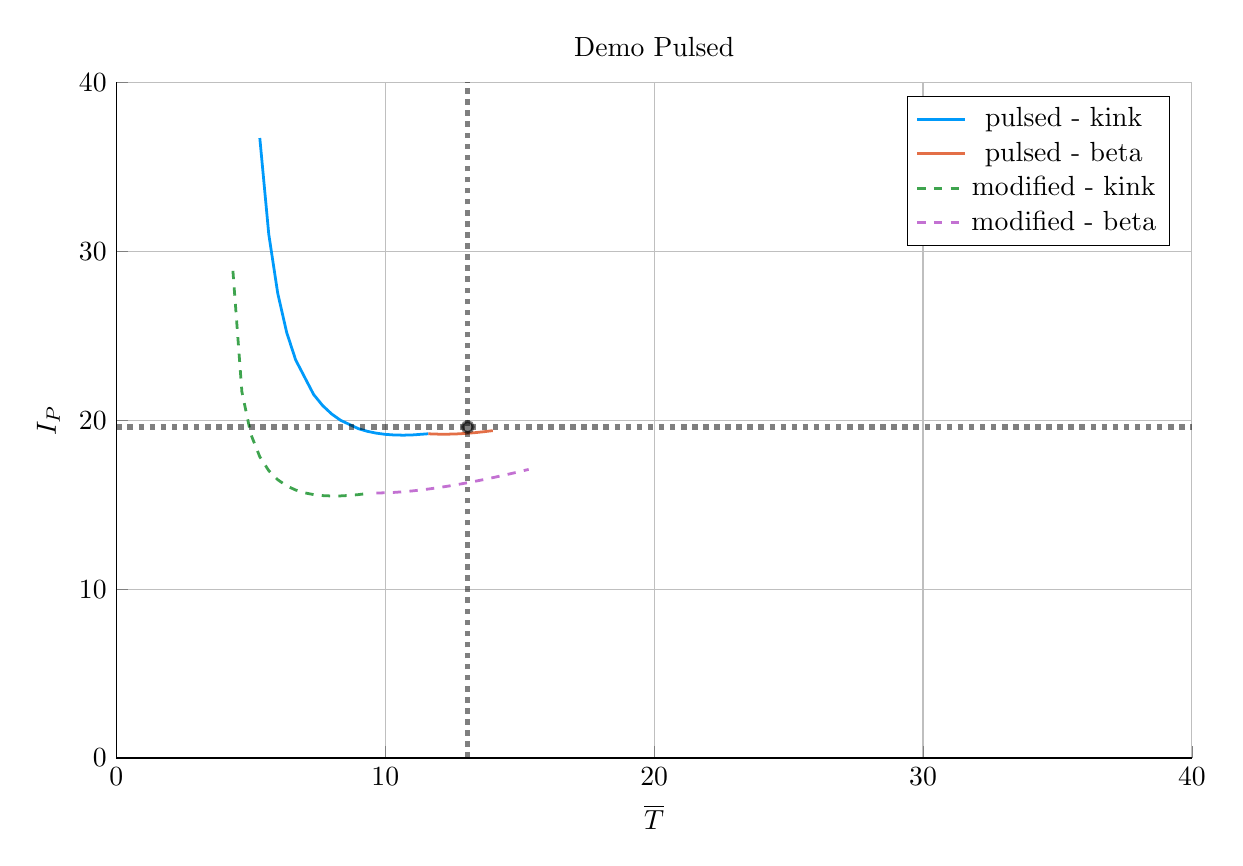
\begin{tikzpicture}[]
\begin{axis}[height = {101.6mm}, ylabel = {$I_P$}, title = {Demo Pulsed}, xmin = {0.0}, xmax = {40.0}, ymax = {40.0}, xlabel = {$\overline T$}, {unbounded coords=jump, scaled x ticks = false, xticklabel style={rotate = 0}, xmajorgrids = true, xtick = {0.0,10.0,20.0,30.0,40.0}, xticklabels = {0,10,20,30,40}, xtick align = inside, axis lines* = left, scaled y ticks = false, yticklabel style={rotate = 0}, ymajorgrids = true, ytick = {0.0,10.0,20.0,30.0,40.0}, yticklabels = {0,10,20,30,40}, ytick align = inside, axis lines* = left,     xshift = 0.0mm,
    yshift = 0.0mm,
    axis background/.style={fill={rgb,1:red,1.00000000;green,1.00000000;blue,1.00000000}}
}, ymin = {0.0}, width = {152.4mm}]\addplot+ [color = {rgb,1:red,0.00000000;green,0.60560316;blue,0.97868012},
draw opacity=1.0,
line width=1,
solid,mark = none,
mark size = 2.0,
mark options = {
    color = {rgb,1:red,0.00000000;green,0.00000000;blue,0.00000000}, draw opacity = 1.0,
    fill = {rgb,1:red,0.00000000;green,0.60560316;blue,0.97868012}, fill opacity = 1.0,
    line width = 1,
    rotate = 0,
    solid
}]coordinates {
(5.333333333333333, 36.71051032912112)
(5.666666666666667, 31.014995367356207)
(6.0, 27.51734786322149)
(6.333333333333333, 25.19534286389616)
(6.666666666666667, 23.57285610926683)
(7.333333333333333, 21.52905816503197)
(7.666666666666667, 20.874444053021588)
(8.0, 20.377542510464334)
(8.333333333333334, 19.99951688957442)
(9.0, 19.499202175706746)
(9.333333333333334, 19.343044014643887)
(9.666666666666666, 19.233955791269285)
(10.0, 19.16365729524907)
(10.333333333333334, 19.125701869840853)
(10.666666666666666, 19.11499858904485)
(11.0, 19.127475979338943)
(11.600962879632572, 19.198383823705257)
};
\addlegendentry{pulsed - kink}
\addplot+ [color = {rgb,1:red,0.88887350;green,0.43564919;blue,0.27812294},
draw opacity=1.0,
line width=1,
solid,mark = none,
mark size = 2.0,
mark options = {
    color = {rgb,1:red,0.00000000;green,0.00000000;blue,0.00000000}, draw opacity = 1.0,
    fill = {rgb,1:red,0.88887350;green,0.43564919;blue,0.27812294}, fill opacity = 1.0,
    line width = 1,
    rotate = 0,
    solid
}]coordinates {
(11.600962879632572, 19.198383823705257)
(11.666666666666666, 19.192414153878335)
(12.0, 19.174087186739918)
(12.333333333333334, 19.17397121853779)
(12.666666666666666, 19.189978018951553)
(13.0, 19.220357277326283)
(13.333333333333334, 19.263633100211838)
(13.666666666666666, 19.31855421750887)
(14.0, 19.384054548489104)
};
\addlegendentry{pulsed - beta}
\addplot+ [color = {rgb,1:red,0.24222430;green,0.64327509;blue,0.30444865},
draw opacity=1.0,
line width=1,
dashed,mark = none,
mark size = 2.0,
mark options = {
    color = {rgb,1:red,0.00000000;green,0.00000000;blue,0.00000000}, draw opacity = 1.0,
    fill = {rgb,1:red,0.24222430;green,0.64327509;blue,0.30444865}, fill opacity = 1.0,
    line width = 1,
    rotate = 0,
    solid
}]coordinates {
(4.333333333333333, 28.845639077165217)
(4.666666666666667, 21.687713986294685)
(5.0, 19.170340224057398)
(5.333333333333333, 17.83397336320386)
(5.666666666666667, 17.01478565989059)
(6.0, 16.477486603636205)
(6.333333333333333, 16.113958654578386)
(6.666666666666667, 15.866460603971907)
(7.0, 15.700928946757587)
(7.333333333333333, 15.59578560596909)
(7.666666666666667, 15.536607983152381)
(8.0, 15.513342675582972)
(8.333333333333334, 15.518740955012225)
(8.666666666666666, 15.547428978968492)
(9.0, 15.595329068459918)
(9.333333333333334, 15.659285368310089)
};
\addlegendentry{modified - kink}
\addplot+ [color = {rgb,1:red,0.76444018;green,0.44411178;blue,0.82429754},
draw opacity=1.0,
line width=1,
dashed,mark = none,
mark size = 2.0,
mark options = {
    color = {rgb,1:red,0.00000000;green,0.00000000;blue,0.00000000}, draw opacity = 1.0,
    fill = {rgb,1:red,0.76444018;green,0.44411178;blue,0.82429754}, fill opacity = 1.0,
    line width = 1,
    rotate = 0,
    solid
}]coordinates {
(9.666666666666666, 15.691192911261952)
(10.0, 15.70165788278533)
(10.333333333333334, 15.726578234093749)
(10.666666666666666, 15.764127054896537)
(11.0, 15.812802650736373)
(11.333333333333334, 15.871360766004056)
(11.666666666666666, 15.938763317563621)
(12.0, 16.014139065408)
(12.333333333333334, 16.09675304572932)
(12.666666666666666, 16.185982524147033)
(13.0, 16.281297862810217)
(13.333333333333334, 16.382247130746602)
(13.666666666666666, 16.488443597982137)
(14.0, 16.5995554722192)
(14.333333333333334, 16.715297396529092)
(14.666666666666666, 16.83542334285969)
(15.0, 16.959720624053933)
(15.333333333333334, 17.088004807739882)
};
\addlegendentry{modified - beta}
\addplot+ [color = {rgb,1:red,0.00000000;green,0.00000000;blue,0.00000000},
draw opacity=0.5,
line width=2,
dotted,mark = none,
mark size = 2.0,
mark options = {
    color = {rgb,1:red,0.00000000;green,0.00000000;blue,0.00000000}, draw opacity = 0.5,
    fill = {rgb,1:red,0.00000000;green,0.00000000;blue,0.00000000}, fill opacity = 0.5,
    line width = 1,
    rotate = 0,
    solid
},forget plot]coordinates {
(0.0, 19.6)
(40.0, 19.6)
};
\addplot+ [color = {rgb,1:red,0.00000000;green,0.00000000;blue,0.00000000},
draw opacity=0.5,
line width=2,
dotted,mark = none,
mark size = 2.0,
mark options = {
    color = {rgb,1:red,0.00000000;green,0.00000000;blue,0.00000000}, draw opacity = 0.5,
    fill = {rgb,1:red,0.00000000;green,0.00000000;blue,0.00000000}, fill opacity = 0.5,
    line width = 1,
    rotate = 0,
    solid
},forget plot]coordinates {
(13.065, 0.0)
(13.065, 40.0)
};
\addplot+[draw=none, color = {rgb,1:red,0.00000000;green,0.00000000;blue,0.00000000},
draw opacity=0.5,
line width=0,
solid,mark = *,
mark size = 2.0,
mark options = {
    color = {rgb,1:red,0.00000000;green,0.00000000;blue,0.00000000}, draw opacity = 0.5,
    fill = {rgb,1:red,0.00000000;green,0.00000000;blue,0.00000000}, fill opacity = 0.5,
    line width = 1,
    rotate = 0,
    solid
},forget plot] coordinates {
(13.065, 19.6)
};
\end{axis}

\end{tikzpicture}

    \end{adjustbox}
        \caption{$I_P$ vs $\overline T$}
    \end{subfigure}
    \hfill \hfill ~\\ ~\\ ~\\
    \caption{Demo Pulsed Model Comparison} ~\\
\end{figure*}

\begin{table}[h!]
\centering  
\caption{Demo Pulsed Variables}
\hfill
\begin{subtable}[t]{0.4\textwidth}
\centering  
\caption{Input Variables} ~\\
\begin{tabular}{ c|c } 

Input            & Value           \\
\hline
$H$              & 1.1             \\
$Q$              & 39.86           \\
$N_{G}$          & 1.2             \\
$\epsilon$       & 0.3226          \\
$\kappa_{95}$    & 1.59            \\
$\delta_{95}$    & 0.333           \\
$\nu_{n}$        & 0.27            \\
$\nu_{T}$        & 1.094           \\
$l_{i}$          & 1.155           \\
$A$              & 2.735           \\
$Z_{eff}$        & 2.584           \\
$f_{D}$          & 0.7753          \\
$\tau_{FT}$      & 7273          \\
$B_{CS}$         & 12.77           \\

\end{tabular}
\end{subtable}
\hfill
\begin{subtable}[t]{0.5\textwidth}
\centering  
\caption{Output Variables} ~\\
\begin{tabular}{ c|c|c } 

Output           & Original         & Fussy.jl        \\
\hline
$R_{0}$          & 9.072            & 8.1             \\
$B_{0}$          & 5.667            & 5.48            \\
$I_{P}$          & 19.6             & 19.26           \\
$\overline n$    & 0.7983           & 0.9795          \\
$\overline T$    & 13.06            & 13.28           \\
$\beta_{N}$       & 0.0259           & 0.0259          \\
$q_{95}$         & 3.247            & 2.853           \\
$P_{W}$          & 1.05             & 1.466           \\
$f_{BS}$         & 0.348            & 0.1637          \\
$f_{CD}$         & 0.096            & 0.1062          \\
$f_{IN}$         & 0.557            & 0.7302          \\
$\volume$         & 2502           & 1751          \\
$P_{F}$          & 2037           & 2376          \\
$\eta_{CD}$      & 0.2721           & -     

\end{tabular}
\end{subtable}
\hfill
\hfill
\end{table}

\section{Developing Prototype Reactors}

\begin{figure}[h!]
\centering
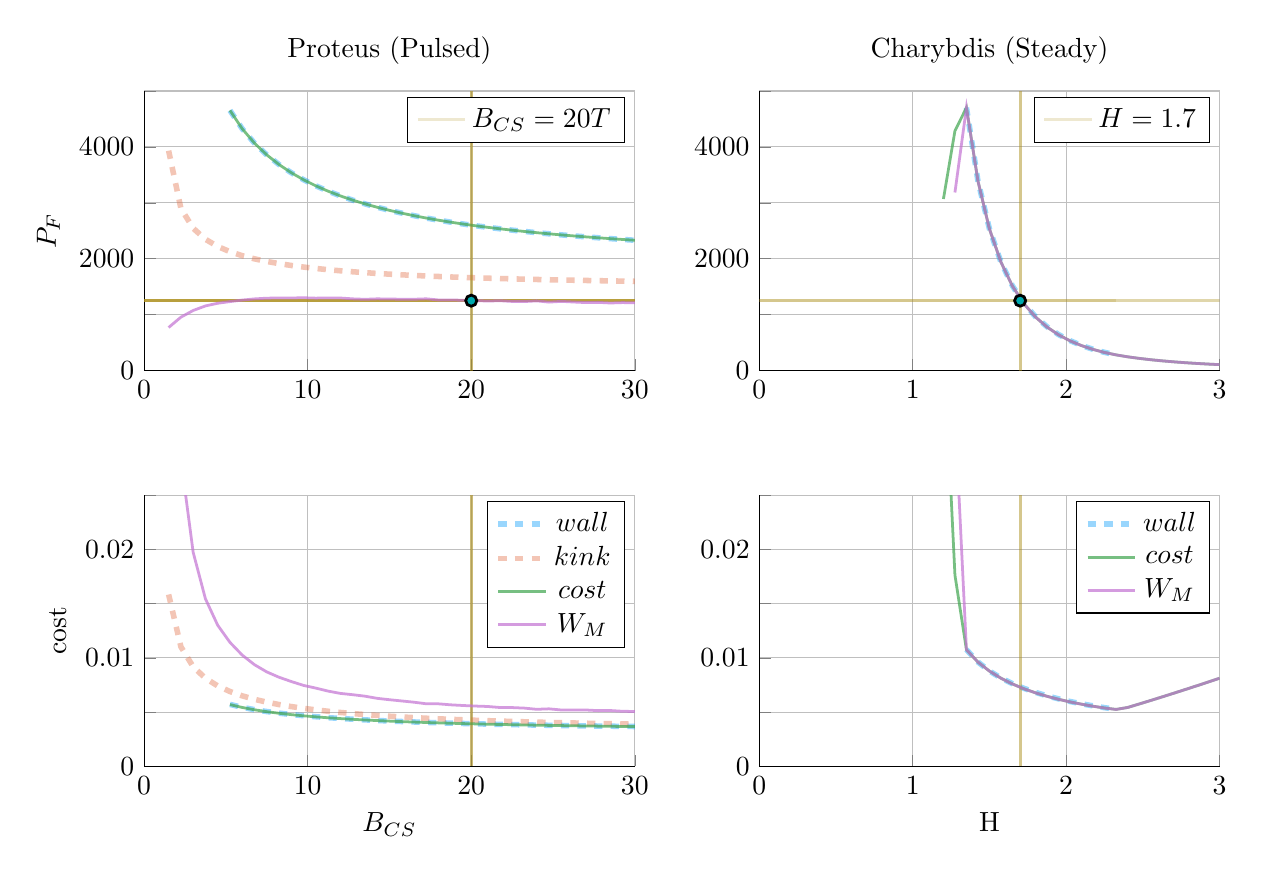
\begin{tikzpicture}[]
\begin{axis}[height = {51.32916666666667mm}, ylabel = {$P_F$}, title = {Proteus (Pulsed)}, xmin = {0}, xmax = {30.0}, ymax = {5000.0}, xlabel = {}, {unbounded coords=jump, scaled x ticks = false, xticklabel style={rotate = 0}, xmajorgrids = true, xtick = {0.0,10.0,20.0,30.0}, xticklabels = {0,10,20,30}, xtick align = inside, axis lines* = left, scaled y ticks = false, yticklabel style={rotate = 0}, ymajorgrids = true, ytick = {0,1000,2000,3000,4000,5000}, yticklabels = {0,,2000,,4000,}, ytick align = inside, axis lines* = left,     xshift = 0.0mm,
    yshift = 50.27mm,
    axis background/.style={fill={rgb,1:red,1.00000000;green,1.00000000;blue,1.00000000}}
}, ymin = {2.220446049250313e-16}, width = {78.14027777777778mm}]\addplot+ [color = {rgb,1:red,0.67554396;green,0.55566233;blue,0.09423434},
draw opacity=0.2,
line width=1,
solid,mark = none,
mark size = 2.0,
mark options = {
    color = {rgb,1:red,0.00000000;green,0.00000000;blue,0.00000000}, draw opacity = 1.0,
    fill = {rgb,1:red,0.67554396;green,0.55566233;blue,0.09423434}, fill opacity = 1.0,
    line width = 1,
    rotate = 0,
    solid
}]coordinates {
(20.0, 2.220446049250313e-16)
(20.0, 5000.0)
};
\addlegendentry{$B_{CS} = 20 T$}
\addplot+ [color = {rgb,1:red,0.67554396;green,0.55566233;blue,0.09423434},
draw opacity=0.2,
line width=1,
solid,mark = none,
mark size = 2.0,
mark options = {
    color = {rgb,1:red,0.00000000;green,0.00000000;blue,0.00000000}, draw opacity = 1.0,
    fill = {rgb,1:red,0.67554396;green,0.55566233;blue,0.09423434}, fill opacity = 1.0,
    line width = 1,
    rotate = 0,
    solid
},forget plot]coordinates {
(0.0, 1250.0)
(30.0, 1250.0)
};
\addplot+[draw=none, color = {rgb,1:red,0.00000048;green,0.66575898;blue,0.68099695},
draw opacity=1.0,
line width=0,
solid,mark = *,
mark size = 2.0,
mark options = {
    color = {rgb,1:red,0.00000000;green,0.00000000;blue,0.00000000}, draw opacity = 1.0,
    fill = {rgb,1:red,0.00000048;green,0.66575898;blue,0.68099695}, fill opacity = 1.0,
    line width = 1,
    rotate = 0,
    solid
},forget plot] coordinates {
(20, 1250)
};
\addplot+ [color = {rgb,1:red,0.67554396;green,0.55566233;blue,0.09423434},
draw opacity=0.2,
line width=1,
solid,mark = none,
mark size = 2.0,
mark options = {
    color = {rgb,1:red,0.00000000;green,0.00000000;blue,0.00000000}, draw opacity = 1.0,
    fill = {rgb,1:red,0.67554396;green,0.55566233;blue,0.09423434}, fill opacity = 1.0,
    line width = 1,
    rotate = 0,
    solid
},forget plot]coordinates {
(0.0, 1250.0)
(30.0, 1250.0)
};
\addplot+ [color = {rgb,1:red,0.00000000;green,0.60560316;blue,0.97868012},
draw opacity=0.4,
line width=2,
dashed,mark = none,
mark size = 2.0,
mark options = {
    color = {rgb,1:red,0.00000000;green,0.00000000;blue,0.00000000}, draw opacity = 1.0,
    fill = {rgb,1:red,0.00000000;green,0.60560316;blue,0.97868012}, fill opacity = 1.0,
    line width = 1,
    rotate = 0,
    solid
},forget plot]coordinates {
(5.25, 4651.734735476011)
(6.0, 4323.6250098364)
(6.75, 4065.99692078527)
(7.5, 3857.273578687972)
(8.25, 3684.1342593418663)
(9.0, 3537.844669896544)
(9.75, 3412.404653539425)
(10.5, 3303.536032694244)
(11.25, 3208.094051273514)
(12.0, 3123.707522754923)
(12.75, 3048.5495054628623)
(13.5, 2981.185980181023)
(14.25, 2920.472987010462)
(15.0, 2865.484885250518)
(15.75, 2815.463186166668)
(16.5, 2769.7793320244814)
(17.25, 2727.9071420752607)
(18.0, 2689.4020933235493)
(18.75, 2653.885520176901)
(19.5, 2621.0324111911764)
(20.25, 2590.561874678777)
(21.0, 2562.2296107375955)
(21.75, 2535.8219099446264)
(22.5, 2511.150826555893)
(23.25, 2488.050264495335)
(24.0, 2466.372779394113)
(24.75, 2445.986947213969)
(25.5, 2426.775184780072)
(26.25, 2408.6319334297787)
(27.0, 2391.4621364565396)
(27.75, 2375.1799557182867)
(28.5, 2359.707684182671)
(29.25, 2344.974819785335)
(30.0, 2330.917272823136)
};
\addplot+ [color = {rgb,1:red,0.67554396;green,0.55566233;blue,0.09423434},
draw opacity=0.2,
line width=1,
solid,mark = none,
mark size = 2.0,
mark options = {
    color = {rgb,1:red,0.00000000;green,0.00000000;blue,0.00000000}, draw opacity = 1.0,
    fill = {rgb,1:red,0.67554396;green,0.55566233;blue,0.09423434}, fill opacity = 1.0,
    line width = 1,
    rotate = 0,
    solid
},forget plot]coordinates {
(20.0, 2.220446049250313e-16)
(20.0, 5000.0)
};
\addplot+ [color = {rgb,1:red,0.67554396;green,0.55566233;blue,0.09423434},
draw opacity=0.2,
line width=1,
solid,mark = none,
mark size = 2.0,
mark options = {
    color = {rgb,1:red,0.00000000;green,0.00000000;blue,0.00000000}, draw opacity = 1.0,
    fill = {rgb,1:red,0.67554396;green,0.55566233;blue,0.09423434}, fill opacity = 1.0,
    line width = 1,
    rotate = 0,
    solid
},forget plot]coordinates {
(0.0, 1250.0)
(30.0, 1250.0)
};
\addplot+ [color = {rgb,1:red,0.67554396;green,0.55566233;blue,0.09423434},
draw opacity=0.2,
line width=1,
solid,mark = none,
mark size = 2.0,
mark options = {
    color = {rgb,1:red,0.00000000;green,0.00000000;blue,0.00000000}, draw opacity = 1.0,
    fill = {rgb,1:red,0.67554396;green,0.55566233;blue,0.09423434}, fill opacity = 1.0,
    line width = 1,
    rotate = 0,
    solid
},forget plot]coordinates {
(0.0, 1250.0)
(30.0, 1250.0)
};
\addplot+ [color = {rgb,1:red,0.88887350;green,0.43564919;blue,0.27812294},
draw opacity=0.4,
line width=2,
dashed,mark = none,
mark size = 2.0,
mark options = {
    color = {rgb,1:red,0.00000000;green,0.00000000;blue,0.00000000}, draw opacity = 1.0,
    fill = {rgb,1:red,0.88887350;green,0.43564919;blue,0.27812294}, fill opacity = 1.0,
    line width = 1,
    rotate = 0,
    solid
},forget plot]coordinates {
(1.5, 3931.6170696070676)
(2.25, 2900.7235747979908)
(3.0, 2544.8446560898715)
(3.75, 2348.228116500571)
(4.5, 2219.0134794713767)
(5.25, 2125.815532966674)
(6.0, 2054.566085735622)
(6.75, 1997.8824990557177)
(7.5, 1951.4633680592258)
(8.25, 1912.6074536455505)
(9.0, 1879.5196356674505)
(9.75, 1850.953068441656)
(10.5, 1826.0101459658863)
(11.25, 1804.02551415983)
(12.0, 1784.493638745381)
(12.75, 1767.0222758941622)
(13.5, 1751.3015387280175)
(14.25, 1737.0827328069474)
(15.0, 1724.1634044428295)
(15.75, 1712.376890482151)
(16.5, 1701.5841921715175)
(17.25, 1691.6685698179294)
(18.0, 1682.530881991843)
(18.75, 1674.0861755860074)
(19.5, 1666.2615100001372)
(20.25, 1658.9932835127363)
(21.0, 1652.2262595201232)
(21.75, 1645.91179207308)
(22.5, 1640.0070406407558)
(23.25, 1634.4738680952948)
(24.0, 1629.2785569006053)
(24.75, 1624.3908184475338)
(25.5, 1619.7835209277835)
(26.25, 1615.432247074283)
(27.0, 1611.314956936522)
(27.75, 1607.4117026157203)
(28.5, 1603.7043856927105)
(29.25, 1600.1765499289672)
(30.0, 1596.813203261599)
};
\addplot+ [color = {rgb,1:red,0.67554396;green,0.55566233;blue,0.09423434},
draw opacity=0.2,
line width=1,
solid,mark = none,
mark size = 2.0,
mark options = {
    color = {rgb,1:red,0.00000000;green,0.00000000;blue,0.00000000}, draw opacity = 1.0,
    fill = {rgb,1:red,0.67554396;green,0.55566233;blue,0.09423434}, fill opacity = 1.0,
    line width = 1,
    rotate = 0,
    solid
},forget plot]coordinates {
(20.0, 2.220446049250313e-16)
(20.0, 5000.0)
};
\addplot+ [color = {rgb,1:red,0.67554396;green,0.55566233;blue,0.09423434},
draw opacity=0.2,
line width=1,
solid,mark = none,
mark size = 2.0,
mark options = {
    color = {rgb,1:red,0.00000000;green,0.00000000;blue,0.00000000}, draw opacity = 1.0,
    fill = {rgb,1:red,0.67554396;green,0.55566233;blue,0.09423434}, fill opacity = 1.0,
    line width = 1,
    rotate = 0,
    solid
},forget plot]coordinates {
(0.0, 1250.0)
(30.0, 1250.0)
};
\addplot+ [color = {rgb,1:red,0.67554396;green,0.55566233;blue,0.09423434},
draw opacity=0.2,
line width=1,
solid,mark = none,
mark size = 2.0,
mark options = {
    color = {rgb,1:red,0.00000000;green,0.00000000;blue,0.00000000}, draw opacity = 1.0,
    fill = {rgb,1:red,0.67554396;green,0.55566233;blue,0.09423434}, fill opacity = 1.0,
    line width = 1,
    rotate = 0,
    solid
},forget plot]coordinates {
(0.0, 1250.0)
(30.0, 1250.0)
};
\addplot+ [color = {rgb,1:red,0.24222430;green,0.64327509;blue,0.30444865},
draw opacity=0.7,
line width=1,
solid,mark = none,
mark size = 2.0,
mark options = {
    color = {rgb,1:red,0.00000000;green,0.00000000;blue,0.00000000}, draw opacity = 1.0,
    fill = {rgb,1:red,0.24222430;green,0.64327509;blue,0.30444865}, fill opacity = 1.0,
    line width = 1,
    rotate = 0,
    solid
},forget plot]coordinates {
(5.25, 4651.856974626446)
(6.0, 4323.626574700689)
(6.75, 4065.9133365013354)
(7.5, 3857.1264771824617)
(8.25, 3683.9377449687768)
(9.0, 3537.608432111376)
(9.75, 3412.1356303067523)
(10.5, 3303.239361854739)
(11.25, 3207.7736468791713)
(12.0, 3123.3664382128795)
(12.75, 3048.1901722862794)
(13.5, 2980.810371417949)
(14.25, 2920.082728006143)
(15.0, 2865.081335141082)
(15.75, 2815.0474968726217)
(16.5, 2769.352491750233)
(17.25, 2727.4700069605415)
(18.0, 2688.955412764386)
(18.75, 2653.4299583736)
(19.5, 2620.5685580410595)
(20.25, 2590.0902617025704)
(21.0, 2561.7507209540713)
(21.75, 2535.3361812985195)
(22.5, 2510.65866319561)
(23.25, 2487.5520396570964)
(24.0, 2465.868837737164)
(24.75, 2445.477613655657)
(25.5, 2426.2607621440256)
(26.25, 2408.1127073411044)
(27.0, 2390.9383771738235)
(27.75, 2374.651919394813)
(28.5, 2359.1756148307045)
(29.25, 2344.438950143004)
(30.0, 2330.377825995788)
};
\addplot+ [color = {rgb,1:red,0.67554396;green,0.55566233;blue,0.09423434},
draw opacity=0.2,
line width=1,
solid,mark = none,
mark size = 2.0,
mark options = {
    color = {rgb,1:red,0.00000000;green,0.00000000;blue,0.00000000}, draw opacity = 1.0,
    fill = {rgb,1:red,0.67554396;green,0.55566233;blue,0.09423434}, fill opacity = 1.0,
    line width = 1,
    rotate = 0,
    solid
},forget plot]coordinates {
(20.0, 2.220446049250313e-16)
(20.0, 5000.0)
};
\addplot+ [color = {rgb,1:red,0.67554396;green,0.55566233;blue,0.09423434},
draw opacity=0.2,
line width=1,
solid,mark = none,
mark size = 2.0,
mark options = {
    color = {rgb,1:red,0.00000000;green,0.00000000;blue,0.00000000}, draw opacity = 1.0,
    fill = {rgb,1:red,0.67554396;green,0.55566233;blue,0.09423434}, fill opacity = 1.0,
    line width = 1,
    rotate = 0,
    solid
},forget plot]coordinates {
(0.0, 1250.0)
(30.0, 1250.0)
};
\addplot+ [color = {rgb,1:red,0.67554396;green,0.55566233;blue,0.09423434},
draw opacity=0.2,
line width=1,
solid,mark = none,
mark size = 2.0,
mark options = {
    color = {rgb,1:red,0.00000000;green,0.00000000;blue,0.00000000}, draw opacity = 1.0,
    fill = {rgb,1:red,0.67554396;green,0.55566233;blue,0.09423434}, fill opacity = 1.0,
    line width = 1,
    rotate = 0,
    solid
},forget plot]coordinates {
(0.0, 1250.0)
(30.0, 1250.0)
};
\addplot+ [color = {rgb,1:red,0.76444018;green,0.44411178;blue,0.82429754},
draw opacity=0.7,
line width=1,
solid,mark = none,
mark size = 2.0,
mark options = {
    color = {rgb,1:red,0.00000000;green,0.00000000;blue,0.00000000}, draw opacity = 1.0,
    fill = {rgb,1:red,0.76444018;green,0.44411178;blue,0.82429754}, fill opacity = 1.0,
    line width = 1,
    rotate = 0,
    solid
},forget plot]coordinates {
(1.5, 770.4535163440595)
(2.25, 954.8730192598816)
(3.0, 1074.7019495723541)
(3.75, 1156.024788273215)
(4.5, 1204.0200711633677)
(5.25, 1233.7948079824048)
(6.0, 1260.6547091987875)
(6.75, 1281.8429530808678)
(7.5, 1294.6082412516207)
(8.25, 1298.1292122440111)
(9.0, 1298.1210010392879)
(9.75, 1302.223238135332)
(10.5, 1295.054060000207)
(11.25, 1299.5652880713872)
(12.0, 1297.6289491073692)
(12.75, 1282.6829774082355)
(13.5, 1274.473146838615)
(14.25, 1282.8743293523935)
(15.0, 1279.4366420169024)
(15.75, 1276.1045609204925)
(16.5, 1275.52105613002)
(17.25, 1283.4690177878747)
(18.0, 1262.712514215648)
(18.75, 1262.7843385038082)
(19.5, 1257.6056644505838)
(20.25, 1251.4051011388665)
(21.0, 1243.4899440635038)
(21.75, 1249.4484707880504)
(22.5, 1236.3207332951713)
(23.25, 1234.0894652277675)
(24.0, 1246.6870760568188)
(24.75, 1224.0642650291306)
(25.5, 1237.4485384154398)
(26.25, 1226.0446362827531)
(27.0, 1215.9720878560222)
(27.75, 1219.8261291156418)
(28.5, 1208.2813208095588)
(29.25, 1215.812124675399)
(30.0, 1211.4870892754757)
};
\end{axis}
\begin{axis}[height = {51.32916666666667mm}, ylabel = {}, title = {Charybdis (Steady)}, xmin = {0}, xmax = {3.0}, ymax = {5000.0}, xlabel = {}, {unbounded coords=jump, scaled x ticks = false, xticklabel style={rotate = 0}, xmajorgrids = true, xtick = {0.0,1.0,2.0,3.0}, xticklabels = {0,1,2,3}, xtick align = inside, axis lines* = left, scaled y ticks = false, yticklabel style={rotate = 0}, ymajorgrids = true, ytick = {0,1000,2000,3000,4000,5000}, yticklabels = {0,,2000,,4000,}, ytick align = inside, axis lines* = left,     xshift = 78.14027777777778mm,
    yshift = 50.27mm,
    axis background/.style={fill={rgb,1:red,1.00000000;green,1.00000000;blue,1.00000000}}
}, ymin = {2.220446049250313e-16}, width = {74.25972222222222mm}]\addplot+ [color = {rgb,1:red,0.67554396;green,0.55566233;blue,0.09423434},
draw opacity=0.2,
line width=1,
solid,mark = none,
mark size = 2.0,
mark options = {
    color = {rgb,1:red,0.00000000;green,0.00000000;blue,0.00000000}, draw opacity = 1.0,
    fill = {rgb,1:red,0.67554396;green,0.55566233;blue,0.09423434}, fill opacity = 1.0,
    line width = 1,
    rotate = 0,
    solid
}]coordinates {
(1.7, 2.220446049250313e-16)
(1.7, 5000.0)
};
\addlegendentry{$H = 1.7$}
\addplot+ [color = {rgb,1:red,0.67554396;green,0.55566233;blue,0.09423434},
draw opacity=0.2,
line width=1,
solid,mark = none,
mark size = 2.0,
mark options = {
    color = {rgb,1:red,0.00000000;green,0.00000000;blue,0.00000000}, draw opacity = 1.0,
    fill = {rgb,1:red,0.67554396;green,0.55566233;blue,0.09423434}, fill opacity = 1.0,
    line width = 1,
    rotate = 0,
    solid
},forget plot]coordinates {
(0.0, 1250.0)
(2.325, 1250.0)
};
\addplot+[draw=none, color = {rgb,1:red,0.00000048;green,0.66575898;blue,0.68099695},
draw opacity=1.0,
line width=0,
solid,mark = *,
mark size = 2.0,
mark options = {
    color = {rgb,1:red,0.00000000;green,0.00000000;blue,0.00000000}, draw opacity = 1.0,
    fill = {rgb,1:red,0.00000048;green,0.66575898;blue,0.68099695}, fill opacity = 1.0,
    line width = 1,
    rotate = 0,
    solid
},forget plot] coordinates {
(1.7, 1250.0)
};
\addplot+ [color = {rgb,1:red,0.00000000;green,0.60560316;blue,0.97868012},
draw opacity=0.4,
line width=2,
dashed,mark = none,
mark size = 2.0,
mark options = {
    color = {rgb,1:red,0.00000000;green,0.00000000;blue,0.00000000}, draw opacity = 1.0,
    fill = {rgb,1:red,0.00000000;green,0.60560316;blue,0.97868012}, fill opacity = 1.0,
    line width = 1,
    rotate = 0,
    solid
},forget plot]coordinates {
(1.35, 4702.419771261358)
(1.425, 3389.739729501066)
(1.5, 2531.7367375233785)
(1.575, 1938.5570892600988)
(1.65, 1513.711721274854)
(1.725, 1200.1687454499686)
(1.8, 964.3328758303221)
(1.875, 784.1982422273053)
(1.95, 644.8519631594907)
(2.025, 535.8348429353653)
(2.1, 449.6995270356)
(2.175, 381.0209603225493)
(2.25, 325.79222945707494)
(2.325, 281.0170460687302)
};
\addplot+ [color = {rgb,1:red,0.67554396;green,0.55566233;blue,0.09423434},
draw opacity=0.2,
line width=1,
solid,mark = none,
mark size = 2.0,
mark options = {
    color = {rgb,1:red,0.00000000;green,0.00000000;blue,0.00000000}, draw opacity = 1.0,
    fill = {rgb,1:red,0.67554396;green,0.55566233;blue,0.09423434}, fill opacity = 1.0,
    line width = 1,
    rotate = 0,
    solid
},forget plot]coordinates {
(1.7, 2.220446049250313e-16)
(1.7, 5000.0)
};
\addplot+ [color = {rgb,1:red,0.67554396;green,0.55566233;blue,0.09423434},
draw opacity=0.2,
line width=1,
solid,mark = none,
mark size = 2.0,
mark options = {
    color = {rgb,1:red,0.00000000;green,0.00000000;blue,0.00000000}, draw opacity = 1.0,
    fill = {rgb,1:red,0.67554396;green,0.55566233;blue,0.09423434}, fill opacity = 1.0,
    line width = 1,
    rotate = 0,
    solid
},forget plot]coordinates {
(0.0, 1250.0)
(3.0, 1250.0)
};
\addplot+ [color = {rgb,1:red,0.24222430;green,0.64327509;blue,0.30444865},
draw opacity=0.7,
line width=1,
solid,mark = none,
mark size = 2.0,
mark options = {
    color = {rgb,1:red,0.00000000;green,0.00000000;blue,0.00000000}, draw opacity = 1.0,
    fill = {rgb,1:red,0.24222430;green,0.64327509;blue,0.30444865}, fill opacity = 1.0,
    line width = 1,
    rotate = 0,
    solid
},forget plot]coordinates {
(1.2, 3068.343606355172)
(1.275, 4286.260736815682)
(1.35, 4701.710701951617)
(1.425, 3388.877819042802)
(1.5, 2531.10959033651)
(1.575, 1938.9724494012169)
(1.65, 1509.401812434612)
(1.725, 1194.4826335617477)
(1.8, 958.6889855821258)
(1.875, 779.1702454071224)
(1.95, 640.597451863543)
(2.025, 532.3571298076668)
(2.1, 446.9177644738313)
(2.175, 378.82904019299)
(2.25, 324.08335892453823)
(2.325, 281.0958675842298)
(2.4, 246.5983680765812)
(2.475, 218.57873818292612)
(2.55, 194.68877419879524)
(2.625, 174.21242277866037)
(2.7, 156.57438414009331)
(2.775, 141.30840500712233)
(2.85, 128.03547590420067)
(2.925, 116.44528649040114)
(3.0, 106.28251642550786)
};
\addplot+ [color = {rgb,1:red,0.67554396;green,0.55566233;blue,0.09423434},
draw opacity=0.2,
line width=1,
solid,mark = none,
mark size = 2.0,
mark options = {
    color = {rgb,1:red,0.00000000;green,0.00000000;blue,0.00000000}, draw opacity = 1.0,
    fill = {rgb,1:red,0.67554396;green,0.55566233;blue,0.09423434}, fill opacity = 1.0,
    line width = 1,
    rotate = 0,
    solid
},forget plot]coordinates {
(1.7, 2.220446049250313e-16)
(1.7, 5000.0)
};
\addplot+ [color = {rgb,1:red,0.67554396;green,0.55566233;blue,0.09423434},
draw opacity=0.2,
line width=1,
solid,mark = none,
mark size = 2.0,
mark options = {
    color = {rgb,1:red,0.00000000;green,0.00000000;blue,0.00000000}, draw opacity = 1.0,
    fill = {rgb,1:red,0.67554396;green,0.55566233;blue,0.09423434}, fill opacity = 1.0,
    line width = 1,
    rotate = 0,
    solid
},forget plot]coordinates {
(0.0, 1250.0)
(3.0, 1250.0)
};
\addplot+ [color = {rgb,1:red,0.76444018;green,0.44411178;blue,0.82429754},
draw opacity=0.7,
line width=1,
solid,mark = none,
mark size = 2.0,
mark options = {
    color = {rgb,1:red,0.00000000;green,0.00000000;blue,0.00000000}, draw opacity = 1.0,
    fill = {rgb,1:red,0.76444018;green,0.44411178;blue,0.82429754}, fill opacity = 1.0,
    line width = 1,
    rotate = 0,
    solid
},forget plot]coordinates {
(1.275, 3184.7544513979055)
(1.35, 4702.336497990941)
(1.425, 3388.9574757185483)
(1.5, 2531.1205717652433)
(1.575, 1938.799888683301)
(1.65, 1508.8938538316263)
(1.725, 1193.8896388912244)
(1.8, 958.1150115203263)
(1.875, 778.6581601462384)
(1.95, 640.1615648471053)
(2.025, 531.9977422035347)
(2.1, 446.62839995026565)
(2.175, 378.60033344126833)
(2.25, 323.90523713971857)
(2.325, 280.72617729356347)
(2.4, 246.59420337797187)
(2.475, 218.57531693530026)
(2.55, 194.6859804122245)
(2.625, 174.2102899084507)
(2.7, 156.57254493780485)
(2.775, 141.30691976562986)
(2.85, 128.0342791712537)
(2.925, 116.44432378465737)
(3.0, 106.2817429069081)
};
\end{axis}
\begin{axis}[height = {50.27083333333333mm}, ylabel = {cost}, xmin = {0}, xmax = {30.0}, ymax = {0.025}, xlabel = {$B_{CS}$}, {unbounded coords=jump, scaled x ticks = false, xticklabel style={rotate = 0}, xmajorgrids = true, xtick = {0.0,10.0,20.0,30.0}, xticklabels = {0,10,20,30}, xtick align = inside, axis lines* = left, scaled y ticks = false, yticklabel style={rotate = 0}, ymajorgrids = true, ytick = {0.0,0.005,0.01,0.015,0.02,0.025}, yticklabels = {0,,0.01,,0.02,}, ytick align = inside, axis lines* = left,     xshift = 0.0mm,
    yshift = 0.0mm,
    axis background/.style={fill={rgb,1:red,1.00000000;green,1.00000000;blue,1.00000000}}
}, ymin = {2.220446049250313e-16}, width = {78.14027777777778mm}]\addplot+ [color = {rgb,1:red,0.67554396;green,0.55566233;blue,0.09423434},
draw opacity=0.2,
line width=1,
solid,mark = none,
mark size = 2.0,
mark options = {
    color = {rgb,1:red,0.00000000;green,0.00000000;blue,0.00000000}, draw opacity = 1.0,
    fill = {rgb,1:red,0.67554396;green,0.55566233;blue,0.09423434}, fill opacity = 1.0,
    line width = 1,
    rotate = 0,
    solid
},forget plot]coordinates {
(20.0, 2.220446049250313e-16)
(20.0, 0.025)
};
\addplot+ [color = {rgb,1:red,0.00000000;green,0.60560316;blue,0.97868012},
draw opacity=0.4,
line width=2,
dashed,mark = none,
mark size = 2.0,
mark options = {
    color = {rgb,1:red,0.00000000;green,0.00000000;blue,0.00000000}, draw opacity = 1.0,
    fill = {rgb,1:red,0.00000000;green,0.60560316;blue,0.97868012}, fill opacity = 1.0,
    line width = 1,
    rotate = 0,
    solid
}]coordinates {
(5.25, 0.005712169507610721)
(6.0, 0.0054444534313977866)
(6.75, 0.005230803362268402)
(7.5, 0.005055242790193239)
(8.25, 0.004907777182901757)
(9.0, 0.0047817748559315625)
(9.75, 0.004672630374322221)
(10.5, 0.004577026917421361)
(11.25, 0.004492503453970045)
(12.0, 0.004417187891782309)
(12.75, 0.004349625699874065)
(13.5, 0.004288666003441743)
(14.25, 0.004233383629634849)
(15.0, 0.004183024392188465)
(15.75, 0.0041369658312621765)
(16.5, 0.0040946884909867755)
(17.25, 0.00405575454151269)
(18.0, 0.004019791621043743)
(18.75, 0.003986480453414949)
(19.5, 0.003955545239870983)
(20.25, 0.003926746118584195)
(21.0, 0.0038998731854889943)
(21.75, 0.0038747417080940948)
(22.5, 0.0038511882607775326)
(23.25, 0.003829067578986908)
(24.0, 0.003808249979473855)
(24.75, 0.0037886192299880117)
(25.5, 0.0037700707786679946)
(26.25, 0.003752510273376433)
(27.0, 0.003735852316365348)
(27.75, 0.003720019411012883)
(28.5, 0.0037049410664172205)
(29.25, 0.003690553032237887)
(30.0, 0.003676796641638663)
};
\addlegendentry{$wall$}
\addplot+ [color = {rgb,1:red,0.67554396;green,0.55566233;blue,0.09423434},
draw opacity=0.2,
line width=1,
solid,mark = none,
mark size = 2.0,
mark options = {
    color = {rgb,1:red,0.00000000;green,0.00000000;blue,0.00000000}, draw opacity = 1.0,
    fill = {rgb,1:red,0.67554396;green,0.55566233;blue,0.09423434}, fill opacity = 1.0,
    line width = 1,
    rotate = 0,
    solid
},forget plot]coordinates {
(20.0, 2.220446049250313e-16)
(20.0, 0.025)
};
\addplot+ [color = {rgb,1:red,0.88887350;green,0.43564919;blue,0.27812294},
draw opacity=0.4,
line width=2,
dashed,mark = none,
mark size = 2.0,
mark options = {
    color = {rgb,1:red,0.00000000;green,0.00000000;blue,0.00000000}, draw opacity = 1.0,
    fill = {rgb,1:red,0.88887350;green,0.43564919;blue,0.27812294}, fill opacity = 1.0,
    line width = 1,
    rotate = 0,
    solid
}]coordinates {
(1.5, 0.015842084276554803)
(2.25, 0.011027723360657306)
(3.0, 0.009184398565447206)
(3.75, 0.008127289094349444)
(4.5, 0.00741869039022264)
(5.25, 0.006901347357456164)
(6.0, 0.006502613319842857)
(6.75, 0.00618357378444017)
(7.5, 0.005921212780220669)
(8.25, 0.005700909685618601)
(9.0, 0.005512859892710094)
(9.75, 0.005350203362180274)
(10.5, 0.005207971705396623)
(11.25, 0.005082463540278267)
(12.0, 0.004970854616305341)
(12.75, 0.004870945672054286)
(13.5, 0.004780993822536362)
(14.25, 0.004699596605104463)
(15.0, 0.004625609671370743)
(15.75, 0.004558089085527066)
(16.5, 0.004496246202265874)
(17.25, 0.00443941766214106)
(18.0, 0.004387039347241793)
(18.75, 0.004338627299893744)
(19.5, 0.004293765577662339)
(20.25, 0.00425209115915401)
(21.0, 0.00421328852908289)
(21.75, 0.004177079626068539)
(22.5, 0.004143219429166407)
(23.25, 0.004111489704198208)
(24.0, 0.004081697424729452)
(24.75, 0.004053669127067244)
(25.5, 0.0040272493764508255)
(26.25, 0.00400229825081617)
(27.0, 0.00397868942182741)
(27.75, 0.003956308530105813)
(28.5, 0.003935051802461753)
(29.25, 0.0039148248692859764)
(30.0, 0.0038955417483358588)
};
\addlegendentry{$kink$}
\addplot+ [color = {rgb,1:red,0.67554396;green,0.55566233;blue,0.09423434},
draw opacity=0.2,
line width=1,
solid,mark = none,
mark size = 2.0,
mark options = {
    color = {rgb,1:red,0.00000000;green,0.00000000;blue,0.00000000}, draw opacity = 1.0,
    fill = {rgb,1:red,0.67554396;green,0.55566233;blue,0.09423434}, fill opacity = 1.0,
    line width = 1,
    rotate = 0,
    solid
},forget plot]coordinates {
(20.0, 2.220446049250313e-16)
(20.0, 0.025)
};
\addplot+ [color = {rgb,1:red,0.24222430;green,0.64327509;blue,0.30444865},
draw opacity=0.7,
line width=1,
solid,mark = none,
mark size = 2.0,
mark options = {
    color = {rgb,1:red,0.00000000;green,0.00000000;blue,0.00000000}, draw opacity = 1.0,
    fill = {rgb,1:red,0.24222430;green,0.64327509;blue,0.30444865}, fill opacity = 1.0,
    line width = 1,
    rotate = 0,
    solid
}]coordinates {
(5.25, 0.005699108286967114)
(6.0, 0.005431918985170679)
(6.75, 0.005218695597593083)
(7.5, 0.00504348909712318)
(8.25, 0.004896322814082233)
(9.0, 0.004770577307210836)
(9.75, 0.0046616558552848835)
(10.5, 0.004566248011640114)
(11.25, 0.00448189757652828)
(12.0, 0.004406736153465555)
(12.75, 0.004339312108727203)
(13.5, 0.004278476921148212)
(14.25, 0.004223307271331157)
(15.0, 0.004173050519899408)
(15.75, 0.004127085500622218)
(16.5, 0.0040848938438373915)
(17.25, 0.004046038614993616)
(18.0, 0.004010148222137879)
(18.75, 0.00397690409614773)
(19.5, 0.003946030963240186)
(20.25, 0.003917289495264197)
(21.0, 0.003890470261769372)
(21.75, 0.003865388865284866)
(22.5, 0.003841882268902024)
(23.25, 0.003819805513198085)
(24.0, 0.003799029152446171)
(24.75, 0.003779437261914396)
(25.5, 0.003760925475183273)
(26.25, 0.0037433996492244382)
(27.0, 0.0037267745723733076)
(27.75, 0.0037109729093953285)
(28.5, 0.0036959243249772844)
(29.25, 0.0036815647050791557)
(30.0, 0.0036678355176402375)
};
\addlegendentry{$cost$}
\addplot+ [color = {rgb,1:red,0.67554396;green,0.55566233;blue,0.09423434},
draw opacity=0.2,
line width=1,
solid,mark = none,
mark size = 2.0,
mark options = {
    color = {rgb,1:red,0.00000000;green,0.00000000;blue,0.00000000}, draw opacity = 1.0,
    fill = {rgb,1:red,0.67554396;green,0.55566233;blue,0.09423434}, fill opacity = 1.0,
    line width = 1,
    rotate = 0,
    solid
},forget plot]coordinates {
(20.0, 2.220446049250313e-16)
(20.0, 0.025)
};
\addplot+ [color = {rgb,1:red,0.76444018;green,0.44411178;blue,0.82429754},
draw opacity=0.7,
line width=1,
solid,mark = none,
mark size = 2.0,
mark options = {
    color = {rgb,1:red,0.00000000;green,0.00000000;blue,0.00000000}, draw opacity = 1.0,
    fill = {rgb,1:red,0.76444018;green,0.44411178;blue,0.82429754}, fill opacity = 1.0,
    line width = 1,
    rotate = 0,
    solid
}]coordinates {
(1.5, 0.05223210501542239)
(2.25, 0.02833040148612962)
(3.0, 0.019732274618891227)
(3.75, 0.015446981617283367)
(4.5, 0.013008492254036925)
(5.25, 0.011429385904544741)
(6.0, 0.010255297100209866)
(6.75, 0.009370308159988431)
(7.5, 0.008707398302373198)
(8.25, 0.008214961790840908)
(9.0, 0.007821656853953102)
(9.75, 0.007463109307240802)
(10.5, 0.0072148694257092635)
(11.25, 0.006938470614651945)
(12.0, 0.006727619695413485)
(12.75, 0.006607789272603787)
(13.5, 0.006472556510230988)
(14.25, 0.006271680008440839)
(15.0, 0.006145123991398349)
(15.75, 0.006031078710959066)
(16.5, 0.005915472007059153)
(17.25, 0.005771538677745611)
(18.0, 0.005766296073041771)
(18.75, 0.005674040666347106)
(19.5, 0.0056123068722334)
(20.25, 0.00556107150454927)
(21.0, 0.005522751053130744)
(21.75, 0.005428199766117318)
(22.5, 0.005421656764476662)
(23.25, 0.005371407215177307)
(24.0, 0.00526158749530259)
(24.75, 0.0053056994490001605)
(25.5, 0.005198962345185956)
(26.25, 0.0052003537942846585)
(27.0, 0.005198849728449561)
(27.75, 0.005140344393809157)
(28.5, 0.005149300170841572)
(29.25, 0.0050795270300204465)
(30.0, 0.0050613944422245455)
};
\addlegendentry{$W_M$}
\end{axis}
\begin{axis}[height = {50.27083333333333mm}, ylabel = {}, xmin = {0}, xmax = {3.0}, ymax = {0.025}, xlabel = {H}, {unbounded coords=jump, scaled x ticks = false, xticklabel style={rotate = 0}, xmajorgrids = true, xtick = {0.0,1.0,2.0,3.0}, xticklabels = {0,1,2,3}, xtick align = inside, axis lines* = left, scaled y ticks = false, yticklabel style={rotate = 0}, ymajorgrids = true, ytick = {0.0,0.005,0.01,0.015,0.02,0.025}, yticklabels = {0,,0.01,,0.02,}, ytick align = inside, axis lines* = left,     xshift = 78.14027777777778mm,
    yshift = 0.0mm,
    axis background/.style={fill={rgb,1:red,1.00000000;green,1.00000000;blue,1.00000000}}
}, ymin = {2.220446049250313e-16}, width = {74.25972222222222mm}]\addplot+ [color = {rgb,1:red,0.67554396;green,0.55566233;blue,0.09423434},
draw opacity=0.2,
line width=1,
solid,mark = none,
mark size = 2.0,
mark options = {
    color = {rgb,1:red,0.00000000;green,0.00000000;blue,0.00000000}, draw opacity = 1.0,
    fill = {rgb,1:red,0.67554396;green,0.55566233;blue,0.09423434}, fill opacity = 1.0,
    line width = 1,
    rotate = 0,
    solid
},forget plot]coordinates {
(1.7, 2.220446049250313e-16)
(1.7, 0.025)
};
\addplot+ [color = {rgb,1:red,0.00000000;green,0.60560316;blue,0.97868012},
draw opacity=0.4,
line width=2,
dashed,mark = none,
mark size = 2.0,
mark options = {
    color = {rgb,1:red,0.00000000;green,0.00000000;blue,0.00000000}, draw opacity = 1.0,
    fill = {rgb,1:red,0.00000000;green,0.60560316;blue,0.97868012}, fill opacity = 1.0,
    line width = 1,
    rotate = 0,
    solid
}]coordinates {
(1.35, 0.010760789339450592)
(1.425, 0.009619732155513792)
(1.5, 0.008790232219442471)
(1.575, 0.008146191975740865)
(1.65, 0.007626898115139337)
(1.725, 0.007192476002664734)
(1.8, 0.006822575452014479)
(1.875, 0.006503593633824443)
(1.95, 0.0062261453756207365)
(2.025, 0.005983128714839427)
(2.1, 0.005769265207076111)
(2.175, 0.005580354114326208)
(2.25, 0.005412981470921174)
(2.325, 0.005264307742085152)
};
\addlegendentry{$wall$}
\addplot+ [color = {rgb,1:red,0.67554396;green,0.55566233;blue,0.09423434},
draw opacity=0.2,
line width=1,
solid,mark = none,
mark size = 2.0,
mark options = {
    color = {rgb,1:red,0.00000000;green,0.00000000;blue,0.00000000}, draw opacity = 1.0,
    fill = {rgb,1:red,0.67554396;green,0.55566233;blue,0.09423434}, fill opacity = 1.0,
    line width = 1,
    rotate = 0,
    solid
},forget plot]coordinates {
(1.7, 2.220446049250313e-16)
(1.7, 0.025)
};
\addplot+ [color = {rgb,1:red,0.24222430;green,0.64327509;blue,0.30444865},
draw opacity=0.7,
line width=1,
solid,mark = none,
mark size = 2.0,
mark options = {
    color = {rgb,1:red,0.00000000;green,0.00000000;blue,0.00000000}, draw opacity = 1.0,
    fill = {rgb,1:red,0.24222430;green,0.64327509;blue,0.30444865}, fill opacity = 1.0,
    line width = 1,
    rotate = 0,
    solid
}]coordinates {
(1.2, 0.03955604782212376)
(1.275, 0.017626268319405003)
(1.35, 0.010752340035232979)
(1.425, 0.009611551048557565)
(1.5, 0.0087828479937872)
(1.575, 0.008128572834245925)
(1.65, 0.007595410831335045)
(1.725, 0.0071543615675789905)
(1.8, 0.006781886166659966)
(1.875, 0.006462738781500925)
(1.95, 0.006186432417976108)
(2.025, 0.0059453885417352845)
(2.1, 0.005733897923299464)
(2.175, 0.0055475060627055185)
(2.25, 0.00538263545086886)
(2.325, 0.005253142678967394)
(2.4, 0.005427786793601137)
(2.475, 0.005746521058004576)
(2.55, 0.006071280283520698)
(2.625, 0.0064016264412292325)
(2.7, 0.0067371256054170785)
(2.775, 0.0070773474574213485)
(2.85, 0.00742187127058562)
(2.925, 0.007770286622950337)
(3.0, 0.00812219532133706)
};
\addlegendentry{$cost$}
\addplot+ [color = {rgb,1:red,0.67554396;green,0.55566233;blue,0.09423434},
draw opacity=0.2,
line width=1,
solid,mark = none,
mark size = 2.0,
mark options = {
    color = {rgb,1:red,0.00000000;green,0.00000000;blue,0.00000000}, draw opacity = 1.0,
    fill = {rgb,1:red,0.67554396;green,0.55566233;blue,0.09423434}, fill opacity = 1.0,
    line width = 1,
    rotate = 0,
    solid
},forget plot]coordinates {
(1.7, 2.220446049250313e-16)
(1.7, 0.025)
};
\addplot+ [color = {rgb,1:red,0.76444018;green,0.44411178;blue,0.82429754},
draw opacity=0.7,
line width=1,
solid,mark = none,
mark size = 2.0,
mark options = {
    color = {rgb,1:red,0.00000000;green,0.00000000;blue,0.00000000}, draw opacity = 1.0,
    fill = {rgb,1:red,0.76444018;green,0.44411178;blue,0.82429754}, fill opacity = 1.0,
    line width = 1,
    rotate = 0,
    solid
}]coordinates {
(1.275, 0.03264708523270401)
(1.35, 0.010753340743983937)
(1.425, 0.00961170510614119)
(1.5, 0.008782873413673694)
(1.575, 0.008128099556360414)
(1.65, 0.007593766537561769)
(1.725, 0.007152108504984691)
(1.8, 0.006779338556104632)
(1.875, 0.006460094676034919)
(1.95, 0.00618382358702477)
(2.025, 0.0059429032795105825)
(2.1, 0.0057315925106183425)
(2.175, 0.005545412165487934)
(2.25, 0.005380765853367499)
(2.325, 0.005248715055615644)
(2.4, 0.00542778246571542)
(2.475, 0.005746516116775585)
(2.55, 0.006071274753887745)
(2.625, 0.006401620641767468)
(2.7, 0.006737118898236894)
(2.775, 0.007077340266624284)
(2.85, 0.007421863685601813)
(2.925, 0.007770278683276702)
(3.0, 0.008122187063544624)
};
\addlegendentry{$W_M$}
\end{axis}

\end{tikzpicture}

\caption{How to Build a Fusion Reactor} ~ \\
\small As is convention in fusion engineering, a good design only relies on one miracle. For steady-state reactors, we assume we can get better confinement -- by increasing $H$. While in the pulsed case, the miracle is assuming strong magnets for the central solenoid -- $B_{CS}$.
\label{fig:circuit_diagram}
\end{figure}

%\end{document}
